%% This file was auto-generated by IPython.
%% Conversion from the original notebook file:
%% stat_AtA_qr.ipynb
%%
\documentclass[11pt,english,fleqn]{article}

%% This is the automatic preamble used by IPython.  Note that it does *not*
%% include a documentclass declaration, that is added at runtime to the overall
%% document.

\usepackage{amsmath}
\usepackage{amssymb}
\usepackage{graphicx}
\usepackage{ucs}
\usepackage[utf8x]{inputenc}

% needed for markdown enumerations to work
\usepackage{enumerate}

% Slightly bigger margins than the latex defaults
\usepackage{geometry}
\geometry{verbose,tmargin=3cm,bmargin=3cm,lmargin=2.5cm,rmargin=2.5cm}

% Define a few colors for use in code, links and cell shading
\usepackage{color}
\definecolor{orange}{cmyk}{0,0.4,0.8,0.2}
\definecolor{darkorange}{rgb}{.71,0.21,0.01}
\definecolor{darkgreen}{rgb}{.12,.54,.11}
\definecolor{myteal}{rgb}{.26, .44, .56}
\definecolor{gray}{gray}{0.45}
\definecolor{lightgray}{gray}{.95}
\definecolor{mediumgray}{gray}{.8}
\definecolor{inputbackground}{rgb}{.95, .95, .85}
\definecolor{outputbackground}{rgb}{.95, .95, .95}
\definecolor{traceback}{rgb}{1, .95, .95}

% Framed environments for code cells (inputs, outputs, errors, ...).  The
% various uses of \unskip (or not) at the end were fine-tuned by hand, so don't
% randomly change them unless you're sure of the effect it will have.
\usepackage{framed}

% remove extraneous vertical space in boxes
\setlength\fboxsep{0pt}

% codecell is the whole input+output set of blocks that a Code cell can
% generate.

% TODO: unfortunately, it seems that using a framed codecell environment breaks
% the ability of the frames inside of it to be broken across pages.  This
% causes at least the problem of having lots of empty space at the bottom of
% pages as new frames are moved to the next page, and if a single frame is too
% long to fit on a page, will completely stop latex from compiling the
% document.  So unless we figure out a solution to this, we'll have to instead
% leave the codecell env. as empty.  I'm keeping the original codecell
% definition here (a thin vertical bar) for reference, in case we find a
% solution to the page break issue.

%% \newenvironment{codecell}{%
%%     \def\FrameCommand{\color{mediumgray} \vrule width 1pt \hspace{5pt}}%
%%    \MakeFramed{\vspace{-0.5em}}}
%%  {\unskip\endMakeFramed}

% For now, make this a no-op...
\newenvironment{codecell}{}

 \newenvironment{codeinput}{%
   \def\FrameCommand{\colorbox{inputbackground}}%
   \MakeFramed{\advance\hsize-\width \FrameRestore}}
 {\unskip\endMakeFramed}

\newenvironment{codeoutput}{%
   \def\FrameCommand{\colorbox{outputbackground}}%
   \vspace{-1.4em}
   \MakeFramed{\advance\hsize-\width \FrameRestore}}
 {\unskip\medskip\endMakeFramed}

\newenvironment{traceback}{%
   \def\FrameCommand{\colorbox{traceback}}%
   \MakeFramed{\advance\hsize-\width \FrameRestore}}
 {\endMakeFramed}

% Use and configure listings package for nicely formatted code
\usepackage{listingsutf8}
\lstset{
  language=python,
  inputencoding=utf8x,
  extendedchars=\true,
  aboveskip=\smallskipamount,
  belowskip=\smallskipamount,
  xleftmargin=2mm,
  breaklines=true,
  basicstyle=\small \ttfamily,
  showstringspaces=false,
  keywordstyle=\color{blue}\bfseries,
  commentstyle=\color{myteal},
  stringstyle=\color{darkgreen},
  identifierstyle=\color{darkorange},
  columns=fullflexible,  % tighter character kerning, like verb
}

% The hyperref package gives us a pdf with properly built
% internal navigation ('pdf bookmarks' for the table of contents,
% internal cross-reference links, web links for URLs, etc.)
\usepackage{hyperref}
\hypersetup{
  breaklinks=true,  % so long urls are correctly broken across lines
  colorlinks=true,
  urlcolor=blue,
  linkcolor=darkorange,
  citecolor=darkgreen,
  }

% hardcode size of all verbatim environments to be a bit smaller
\makeatletter 
\g@addto@macro\@verbatim\small\topsep=0.5em\partopsep=0pt
\makeatother 

% Prevent overflowing lines due to urls and other hard-to-break entities.
\sloppy

\setlength{\mathindent}{0pt}
\setlength{\parindent}{0pt}
\setlength{\parskip}{8pt}
\begin{document}

\section{Paralel Matris Çarpımı, Ax, ve QR}

Matris Çarpımı adli yazi tek makinali ortamda matris carpiminin nasil
yapilacagini, ve nasilgorulecebilegini anlatti. Satir bakis acisi, kolon
bakis acisi islendi. Parallel (Hadoop), esle/indirge ortaminda matris
carpimini nasil yapariz? Mesela $A^TA$'yi ele alalim. Bu carpim oldukca
onemli cunku baska sonuclar icin de kullanilabiliyor. Mesela $A$
uzerinde $QR$ ayristirmasi yapmak isterseniz (bkz. Lineer Cebir ders
notlarimiz) bu carpim kullanilabiliyor.

Nasil? QR ayristirmasi kolonlarin hepsi bilindigi gibi birbirine dik
(orthogonal) birim vektorler olan bir $Q$ matrisi ve ust ucgensel (upper
triangular) bir $R$ matrisi olusturur. Ayristirmanin $A^TA$ ile
baglantisi nedir? Eger $A$ yerine onun ayristirmasini $QR$ koyarsak,
\[
A^TA = (QR)^T (QR) = R^T Q^T QR
\]
Tum $Q$ vektorleri birbirine dik, ve birim vektorler ise, $Q^T Q$ birim
matrisi $I$ olur. O zaman
\[
R^T Q^T QR = R^T R
\]
Yani
\[
A^TA = R^TR
\]
Bu muthis bir sonuc. Demek ki $A^TA$ carpimini yaptigimiz anda, bir
yandan $R^TR$ carpim sonucunu da hesaplamis oluyoruz.

Peki $A^TA$ hesaplayip (boylece $R^TR$'yi elde edince) onun icinden
$R$'yi nasil cekip cikartiriz?

Simdi Cholesky ayristirmasi kullanmanin zamani. Cholesky ayristirmasi
(herhangi bir $A$ matrisi uzerinde)
\[A = LL^T\]
olarak bilinir, yani bir matris alt ucgensel (lower triangular -ki L
harfi oradan geliyor-) $L$ matrisine ve onun devrigi olan ust ucgensel
$L^T$'nin carpimina ayristirilir. Elimizde $R^TR$ var, ve ona benzer
$LL^T$ var, $R$ bilindigi gibi ust ucgensel, $L$ alt ucgensel, $L^T$ ve
$R$ birbirine esit demek ki.

Yani $A^TA$ uzerinde numerik hesap kutuphenimzin Cholesky cagrisi
kullanmak bize $QR$'in $R$'sini verir.

Su anda akla su soru gelebilir: madem kutuphane cagrisi yaptik, niye $A$
uzerinde kutuphenimizin $QR$ cagrisini kullanmiyoruz?

Cevap Buyuk Veri argumaninda sakli. Bu ortamda ugrasilan verilerde $A$
matrisi $m \times n$ boyutlarindadir, ve $m$ milyonlar, hatta
milyarlarca satir olabilir. Simdilik $m >> n$ oldugunu farzedelim, yani
$m$, $n$'den ``cok, cok buyuk'', yani ``boyut kolonlarinin'', ki $n$,
sayisi binler ya da onbinlerde. Bu gayet tipik bir senaryo aslinda,
olcum noktalari (boyutlar) var, ama cok fazla degil, diger yandan o
olcumler icin milyonlarca veri noktasi toplanmis. Tipik bir asiri
belirtilmis (overdetermined) sistem - ki en az kareler (least squares)
gibi yaklasimlarin temel aldigi sistemler bunlardir, eldeki denklem
sayisindan daha fazla olcum noktasi vardir. Bu arada en az karelerden
bahsettik, $QR$'in kullanildigi alanlardan biri en az karelerin
cozumudur.

Argumana devam ediyoruz, kutuphane qr cagrisini $A$ uzerinde yaparsak,
$m \times n$ gibi devasa bir matris uzerinde islem yapmak gerekir. Ama
$A^TA$ uzerinde islem (Cholesky) yaparsak, ki bu carpimin boyutu
$n \times m \cdot m \times n = n \times n$, yani cok daha ufak bir
matristir. $A^TA$'in islem bedeli cok ufak, birazdan anlatacagimiz
yontem sayesinde bu bedel $O(m)$.

\subsection{Paralel $A^TA$}

Paralel $A^TA$ carpimina gelelim. Oncelikle elimizdeki becerilere
(capabilities) bakalim. Hadoop ortami bize asiri buyuk bir dosyayi
otomatik olarak makinalara paylastirmamizi ve bir hesap yapilmasi
gerektigine o hesabin elindeki veri parcasi uzerinde islem yapmasini
sagliyor. $A^TA$ orneginde eldeki veri $A$ ve ``cok olan'' $A$'nin
satirlari, yani $m \times n$ boyutlarinda matris var ve $m$ cok buyuk.
Bir $A$ dosyasi tipik olarak soyle gozukecek:

\begin{codecell}
\begin{codeinput}
\begin{lstlisting}
!head -5 A_matrix
\end{lstlisting}
\end{codeinput}
\begin{codeoutput}
\begin{verbatim}
3 4 5 6
3 4 5 2
3 6 7 8
2 2 2 2
9 9 3 3
\end{verbatim}
\end{codeoutput}
\end{codecell}
\begin{codecell}
\begin{codeinput}
\begin{lstlisting}
$A^TA$ carpimini nasil paralelize ederiz? Eger carpima satir bakisini hatirlarsak,

\end{lstlisting}
\end{codeinput}
\end{codecell}
\begin{codecell}
\begin{codeinput}
\begin{lstlisting}
im=imread("AtA.png"); imshow(im)
\end{lstlisting}
\end{codeinput}
\begin{codeoutput}
\begin{verbatim}
<matplotlib.image.AxesImage at 0x2f6d950>
\end{verbatim}
\begin{center}
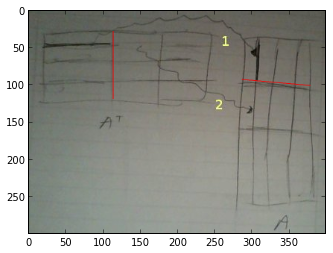
\includegraphics[width=0.7\textwidth]{stat_AtA_qr_files/stat_AtA_qr_fig_00.png}
\par
\end{center}
\end{codeoutput}
\end{codecell}
\end{document}
